\documentclass[oneside,openany]{tietreport}

% Import images and graphics
\usepackage{graphicx}
\usepackage{booktabs}
\usepackage{float}

% Bibliography configuration (Matching TIET template: Biber backend, alphabetic style)
\usepackage[
  date=year,
  style=alphabetic,
  backend=biber,
  sorting=nty,
  maxnames=5,
  minnames=3,
  maxalphanames=4,
  minalphanames=3,
  backref=true,
  doi=false,
  isbn=false,
  url=false,
  eprint=false
]{biblatex}
\addbibresource{references.bib}

%% ==================================================
%% CUSTOMIZE THESE FIELDS FOR YOUR PROJECT
%% ==================================================

% Course/Lab header
% [REPLACE IF NEEDED: Course Code & Course Title]
\TitlePageHeader{%
  UCS 503 - Software Engineering%
}

% Main project title
\ProjectTitle{%
  ProjNaN%
}

% Subtitle or project description
\ProjectSubTitle{%
  An Educational Collaborative Project Management and Contribution Verification Platform%
}

% Student information (up to 4 students)
% [REPLACE PLACEHOLDERS: Roll numbers and Student Names]
\author{%
  \texttt{1024160114} Vanshaj Sharma \\
  \texttt{1024160100} Aryan Thakkar%
}

% Group number, degree, year, program
% [REPLACE PLACEHOLDER: Group Number, e.g., Group: G-14]
\TitlePageSubText{%
  Group: \texttt{\textbf{3P14}} BE Third Year, CSE%
}

% Faculty advisor/guide name
% [REPLACE PLACEHOLDER: Faculty Guide Name]
\AdvisorName{%
  Dr. Anushka%
}

% Evaluation period and department info
\TitlePageFooterText{{%
    \large Mid-Semester Evaluation \\[0.2cm]
    \bfseries Computer Science and Engineering
    Department%
  } \\[0.15cm]
  Thapar Institute of Engineering and Technology,
  Patiala%
}
\raggedbottom

\begin{document}

% Generate title page
\maketitle

% Table of contents (auto-generated from chapters)
\tableofcontents

% ===== CHAPTER 1: INTRODUCTION =====

\chapter{Introduction}

\section{Background and Context}
In undergraduate computer science and software engineering curricula, project-based learning (PBL) serves as a primary pedagogical methodology. Students collaborate in small teams to design, architect, and implement non-trivial software systems over multi-week laboratory modules or semester-long capstone courses~\cite{sommerville2015}.

While collaborative development fosters teamwork and exposes students to modern software engineering lifecycles~\cite{pressman2019}, evaluating student group work presents persistent operational challenges. In conventional academic workflows, course instructors evaluate progress primarily through periodic presentations, status reports, or final code submissions. Consequently, instructors often lack direct, continuous visibility into individual developer participation, branch management, and task completion authenticity.

\textit{ProjNaN} is an educational web platform designed to improve visibility and accountability in student software projects. Unlike enterprise project management software that focuses strictly on corporate workflows, ProjNaN aligns academic course organization (faculty mentors, enrolled classes, automatically generated unique class codes, student teams) with software development workflows (version control telemetry, task state machines, internal rule-based heuristic verification, and contribution accounting).

\subsection{Problem Statement}
Academic evaluation of collaborative student software projects faces three distinct challenges:
\begin{enumerate}
  \item \textbf{Unequal Contribution Distribution}: Group grading models often conceal unequal work distribution. More active students may complete the majority of the implementation while disengaged team members receive unearned credit due to a lack of individual contribution auditing.
  \item \textbf{Evaluation Opacity}: Faculty mentors frequently evaluate final deliverables without granular visibility into code authorship, commit regularity, or technical evidence. Instructors cannot easily determine whether a task was completed by the assigned student or simply marked complete without supporting implementation.
  \item \textbf{Tooling Fragmentation}: Students and instructors typically rely on disconnected tools---enterprise issue trackers uncoupled from academic course rosters, GitHub for repository hosting, and institutional learning management systems (LMS) for grading. This separation introduces administrative overhead and prevents automated correlation between student task completion and repository activity.
\end{enumerate}

\section{Project Objectives}
The core objectives of the ProjNaN platform are formulated under the SMART (Specific, Measurable, Achievable, Relevant, Time-bound) framework:
\begin{enumerate}
  \item \textbf{Objective 1: Role-Based Academic Management}: Implement a role-based access control architecture distinguishing \texttt{teacher} and \texttt{student} roles, supporting automatically generated unique class codes, student self-enrollment, and isolated project workspaces.
  \item \textbf{Objective 2: Repository Telemetry and Heuristic Task Verification}: Implement an automated GitHub synchronization pipeline that ingests remote commits, pull requests, and issues~\cite{githubapi2024}, coupled with an internal rule-based heuristic evaluator that inspects student evidence (PR references and commit hashes) and computes an objective confidence score ($0.00$ to $1.00$) prior to instructor review.
  \item \textbf{Objective 3: Idempotent Contribution Ledger and Team Analytics}: Design an idempotent contribution engine that prevents duplicate XP or point credits across repeated sync events, and aggregate verified activity into quantifiable team effort distribution visualizations (stacked percentage bars) and 14-day velocity charts.
\end{enumerate}

% ===== CHAPTER 2: METHODOLOGY & DESIGN =====

\chapter{Methodology and Design}

\section{System Architecture}
ProjNaN is structured as a tiered client-server web architecture partitioned into four distinct layers: a presentation layer, an API gateway and security layer, a domain service layer, and a relational persistence layer. While SQLite serves as the primary local persistence layer operating with Write-Ahead Logging~\cite{sqlite2024}, the system interfaces with the external GitHub REST API v3 as a secondary external cloud service for source code telemetry.

\subsection{High-Level Design}
The interaction between system actors and functional boundaries is modeled in the Use Case Diagram depicted in Figure~\ref{fig:usecase}.

\begin{figure}[!htbp]
  \centering
  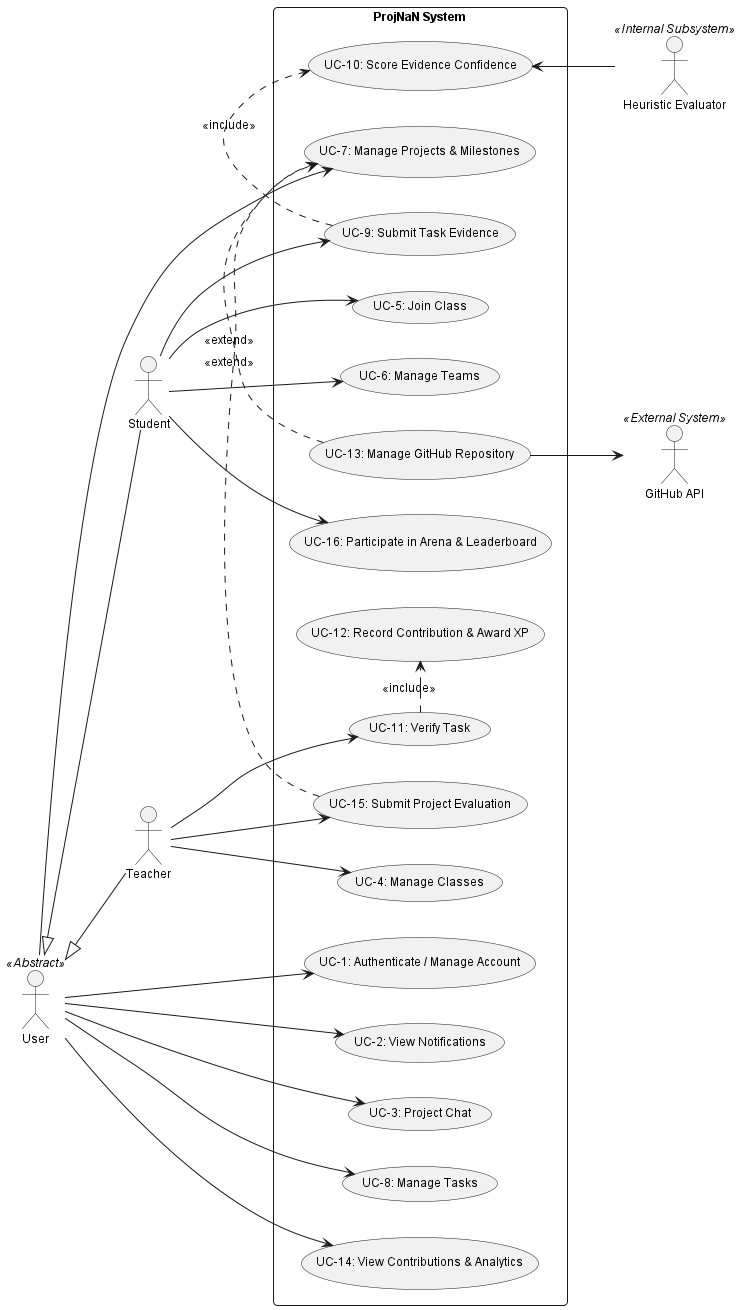
\includegraphics[width=0.95\textwidth]{diagrams/usecase.png}
  \caption{ProjNaN System Use Case Diagram}
  \label{fig:usecase}
\end{figure}

The diagram illustrates the functional boundary of the ProjNaN platform, showing the abstract \texttt{User} actor inherited by \texttt{Student} and \texttt{Teacher}, alongside the external \texttt{GitHub API} and internal \texttt{Heuristic Evaluator} subsystems. It highlights mandatory \texttt{<<include>>} relationships for task evidence confidence scoring and contribution XP attribution, as well as optional \texttt{<<extend>>} branches for repository synchronization and project evaluation.

\subsection{Technical Stack}
The platform implementation is built using open-source libraries and runtimes, interacting with the external GitHub API for telemetry:

\begin{itemize}
  \item \textbf{Framework/Language:} React 19 (\texttt{v19.2.8})~\cite{react2024} with React Router DOM (\texttt{v7.18.2}) on the frontend; Node.js (\texttt{v24.21.0} LTS) executing native ECMAScript Modules with Express.js (\texttt{v4.21.2})~\cite{express2024} on the backend.
  \item \textbf{Database:} Embedded SQLite database managed via Node.js native \texttt{node:sqlite} (\texttt{DatabaseSync}) operating with Write-Ahead Logging (\texttt{WAL}) and enforced foreign key constraints.
  \item \textbf{Tools:} Vite (\texttt{v8.2.0})~\cite{vite2024} for client bundling, Node.js native test runner (\texttt{node:test}), and Supertest (\texttt{v7.0.0}) for automated API assertions.
  \item \textbf{Libraries:} \texttt{bcryptjs} for cryptographic password hashing (10 salt rounds), \texttt{jsonwebtoken} for stateless HMAC-SHA256 bearer session tokens~\cite{jwt2015}, and custom sliding-window rate-limiting and XSS-sanitization middleware.
\end{itemize}

\section{Implementation Details}

\subsection{Module 1: Core Functionality}
The core domain is structured around the relational schema illustrated in the Class Diagram in Figure~\ref{fig:class}.

\begin{figure}[!htbp]
  \centering
  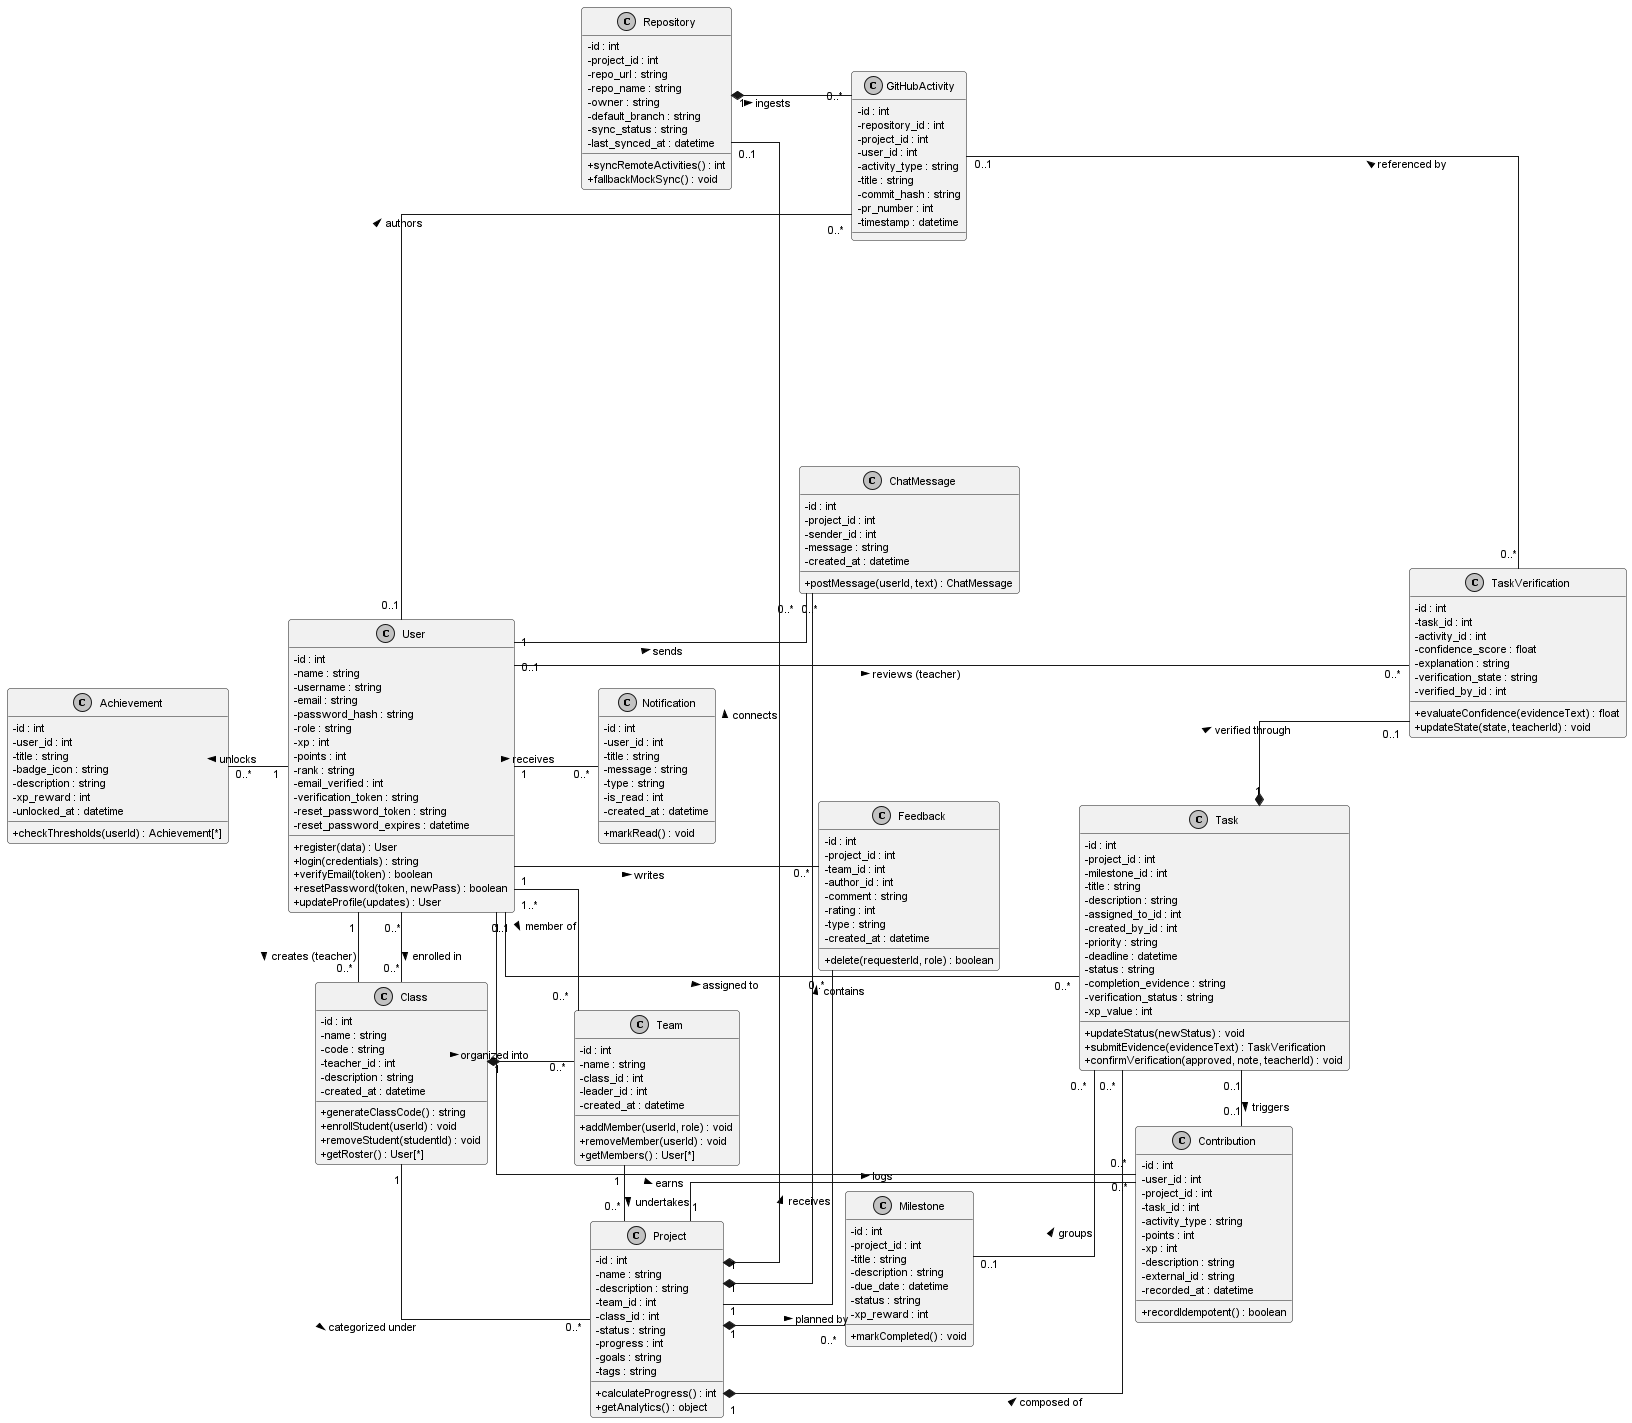
\includegraphics[width=0.98\textwidth]{diagrams/class-diagram.png}
  \caption{ProjNaN Core Domain Class Diagram}
  \label{fig:class}
\end{figure}

Figure~\ref{fig:class} models the 14 core domain entities implemented in the SQLite database and backend service layer. The diagram highlights structural composition between \texttt{Project} and \texttt{Task} ($0..*$), associations connecting \texttt{User} to \texttt{Class} and \texttt{Team}, the link between \texttt{Task} and \texttt{TaskVerification}, and the idempotent reference key (\texttt{external\_id}) in \texttt{Contribution}.

\subsubsection{1. Authentication, RBAC, and Academic Scoping}
User identity is managed in the \texttt{users} table with role validation constrained strictly to \texttt{teacher} or \texttt{student}. Registration generates random 64-hex email verification tokens, and password reset requests enforce a 1-hour expiration window with regex complexity checks. Faculty instantiate academic classes, which automatically generate unique join codes (e.g., \texttt{CS101-ABCD}). Project queries are strictly filtered by authenticated relationships, preventing data leakage across unrelated student teams.

\subsubsection{2. Task Lifecycle and Internal Heuristic Verification}
Tasks transition through four defined states: \texttt{Planned} $\rightarrow$ \texttt{In Progress} $\rightarrow$ \texttt{Verification Pending} $\rightarrow$ \texttt{Completed}. When a student submits completion evidence, the internal rule-based heuristic evaluator analyzes the submission using a deterministic scoring formula:
\begin{equation}
  S_{\text{confidence}} = S_{\text{base}} + \delta_{\text{len}} + \delta_{\text{PR}} + \delta_{\text{commit}}
\end{equation}
where $S_{\text{base}} = 0.50$ (baseline confidence for non-empty text), $\delta_{\text{len}} = 0.15$ for descriptive explanations ($>30$ characters), $\delta_{\text{PR}} = 0.25$ for matching ingested pull requests in the project's \texttt{github\_activities} table (or $+0.10$ for unverified regex matches), and $\delta_{\text{commit}} = 0.20$ for valid commit SHA hashes. Final verification confirmation is restricted strictly to teachers (\texttt{authorizeRoles('teacher')}), which awards XP and points upon approval.

The dynamic interaction between student, frontend, backend controllers, internal heuristic evaluator, and teacher is detailed in the Sequence Diagram in Figure~\ref{fig:taskseq}.

\begin{figure}[!htbp]
  \centering
  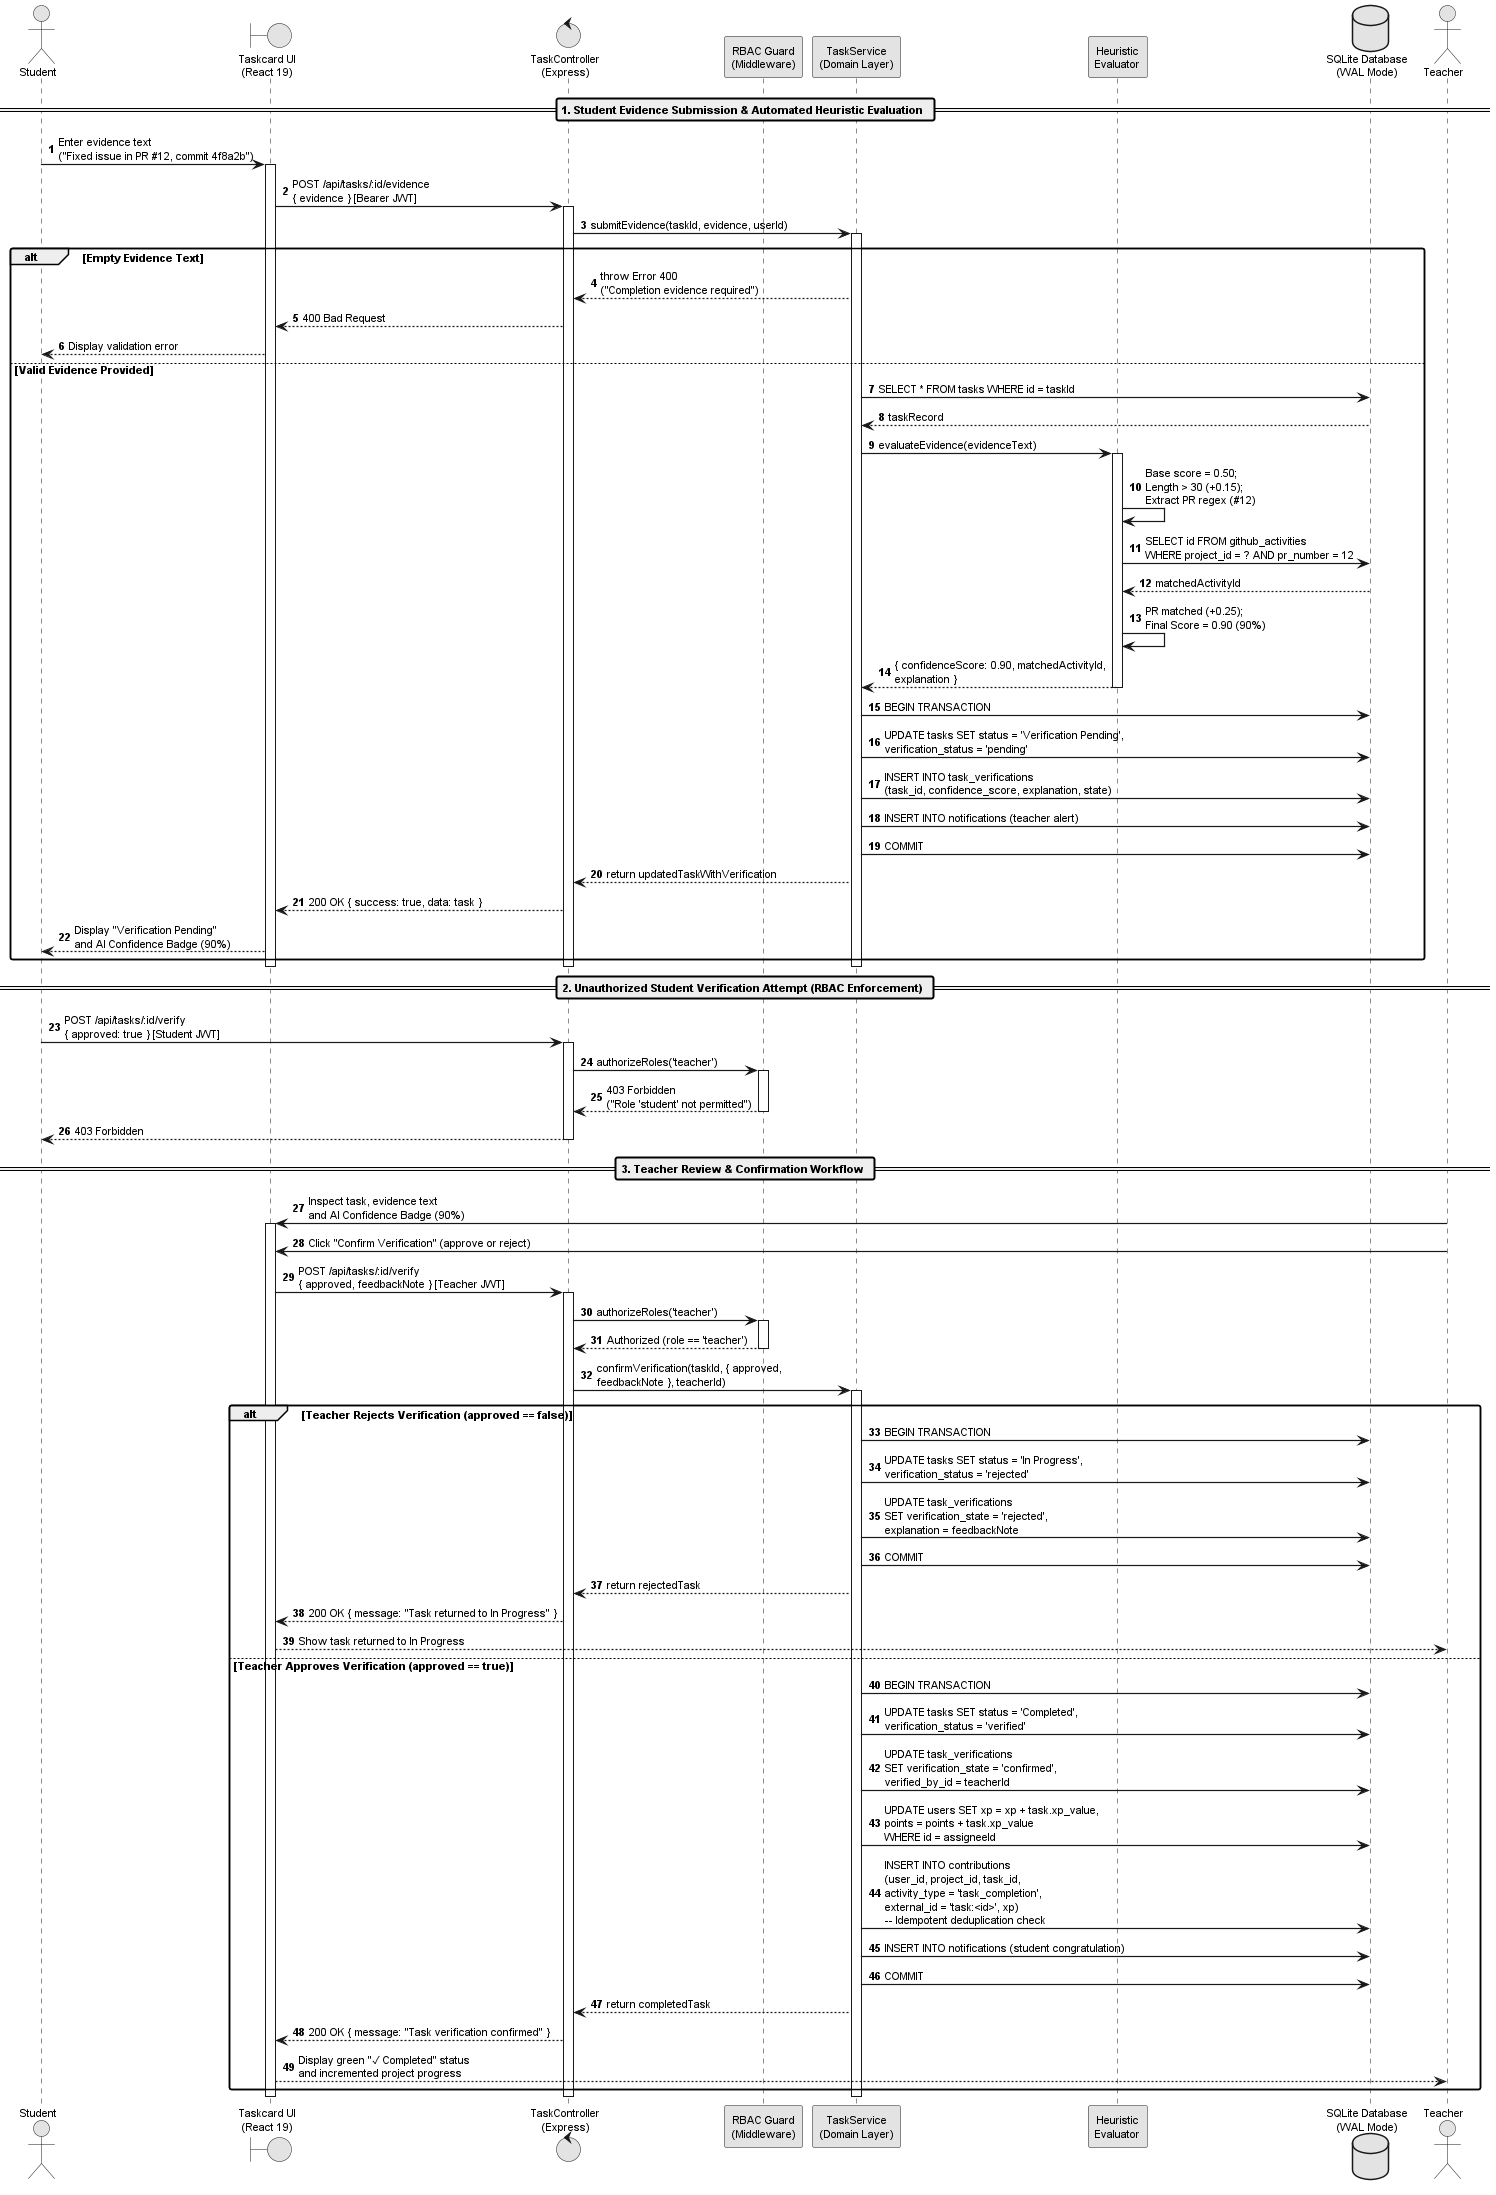
\includegraphics[width=0.95\textwidth]{diagrams/task-verification-sequence.png}
  \caption{Sequence Diagram of Task Evidence Submission, Heuristic Scoring, and Teacher Verification}
  \label{fig:taskseq}
\end{figure}

Figure~\ref{fig:taskseq} traces the chronological message exchanges between the Student, Taskcard UI, TaskController, TaskService, internal Heuristic Evaluator, SQLite Database, and Teacher. It documents the internal query against \texttt{github\_activities}, the RBAC guard intercepting unauthorized student verification attempts (returning HTTP 403), and the atomic database transaction executed upon teacher approval.

\subsection{Module 2: Secondary Features}

\subsubsection{1. GitHub Telemetry Synchronization}
Repositories link to projects via GitHub URLs. The backend synchronizes remote commits, pull requests, and issues via GitHub REST API v3~\cite{githubapi2024}. When remote connections are offline or rate-limited, an automated fallback engine generates realistic synthetic telemetry to preserve system usability and automated test execution.

\subsubsection{2. Team Contribution Engine and Velocity Analytics}
The platform records every verified activity in an idempotent ledger (\texttt{contributions}). The ledger enforces idempotency via a unique index on \texttt{external\_id}, preventing duplicate credits across repeated sync calls. The analytics service calculates individual contribution shares:
\begin{equation}
  P_i = \left( \frac{C_i}{\sum_{k=1}^N C_k} \right) \times 100
\end{equation}
where $C_i$ represents the verified contributions of member $i$. This distribution is rendered in the frontend via stacked effort distribution bars alongside 14-day velocity sparklines.

\subsubsection{3. Gamification and Persistent Notifications}
Students unlock achievement badges (e.g., \textit{First Step}, \textit{Active Contributor}, \textit{Gladiator}) based on verified activity thresholds. A persistent notification service alerts students to instructor evaluations and task verification approvals.

The operational flow of the verification lifecycle is modeled in the Activity Diagram in Figure~\ref{fig:activity}.

\begin{figure}[!htbp]
  \centering
  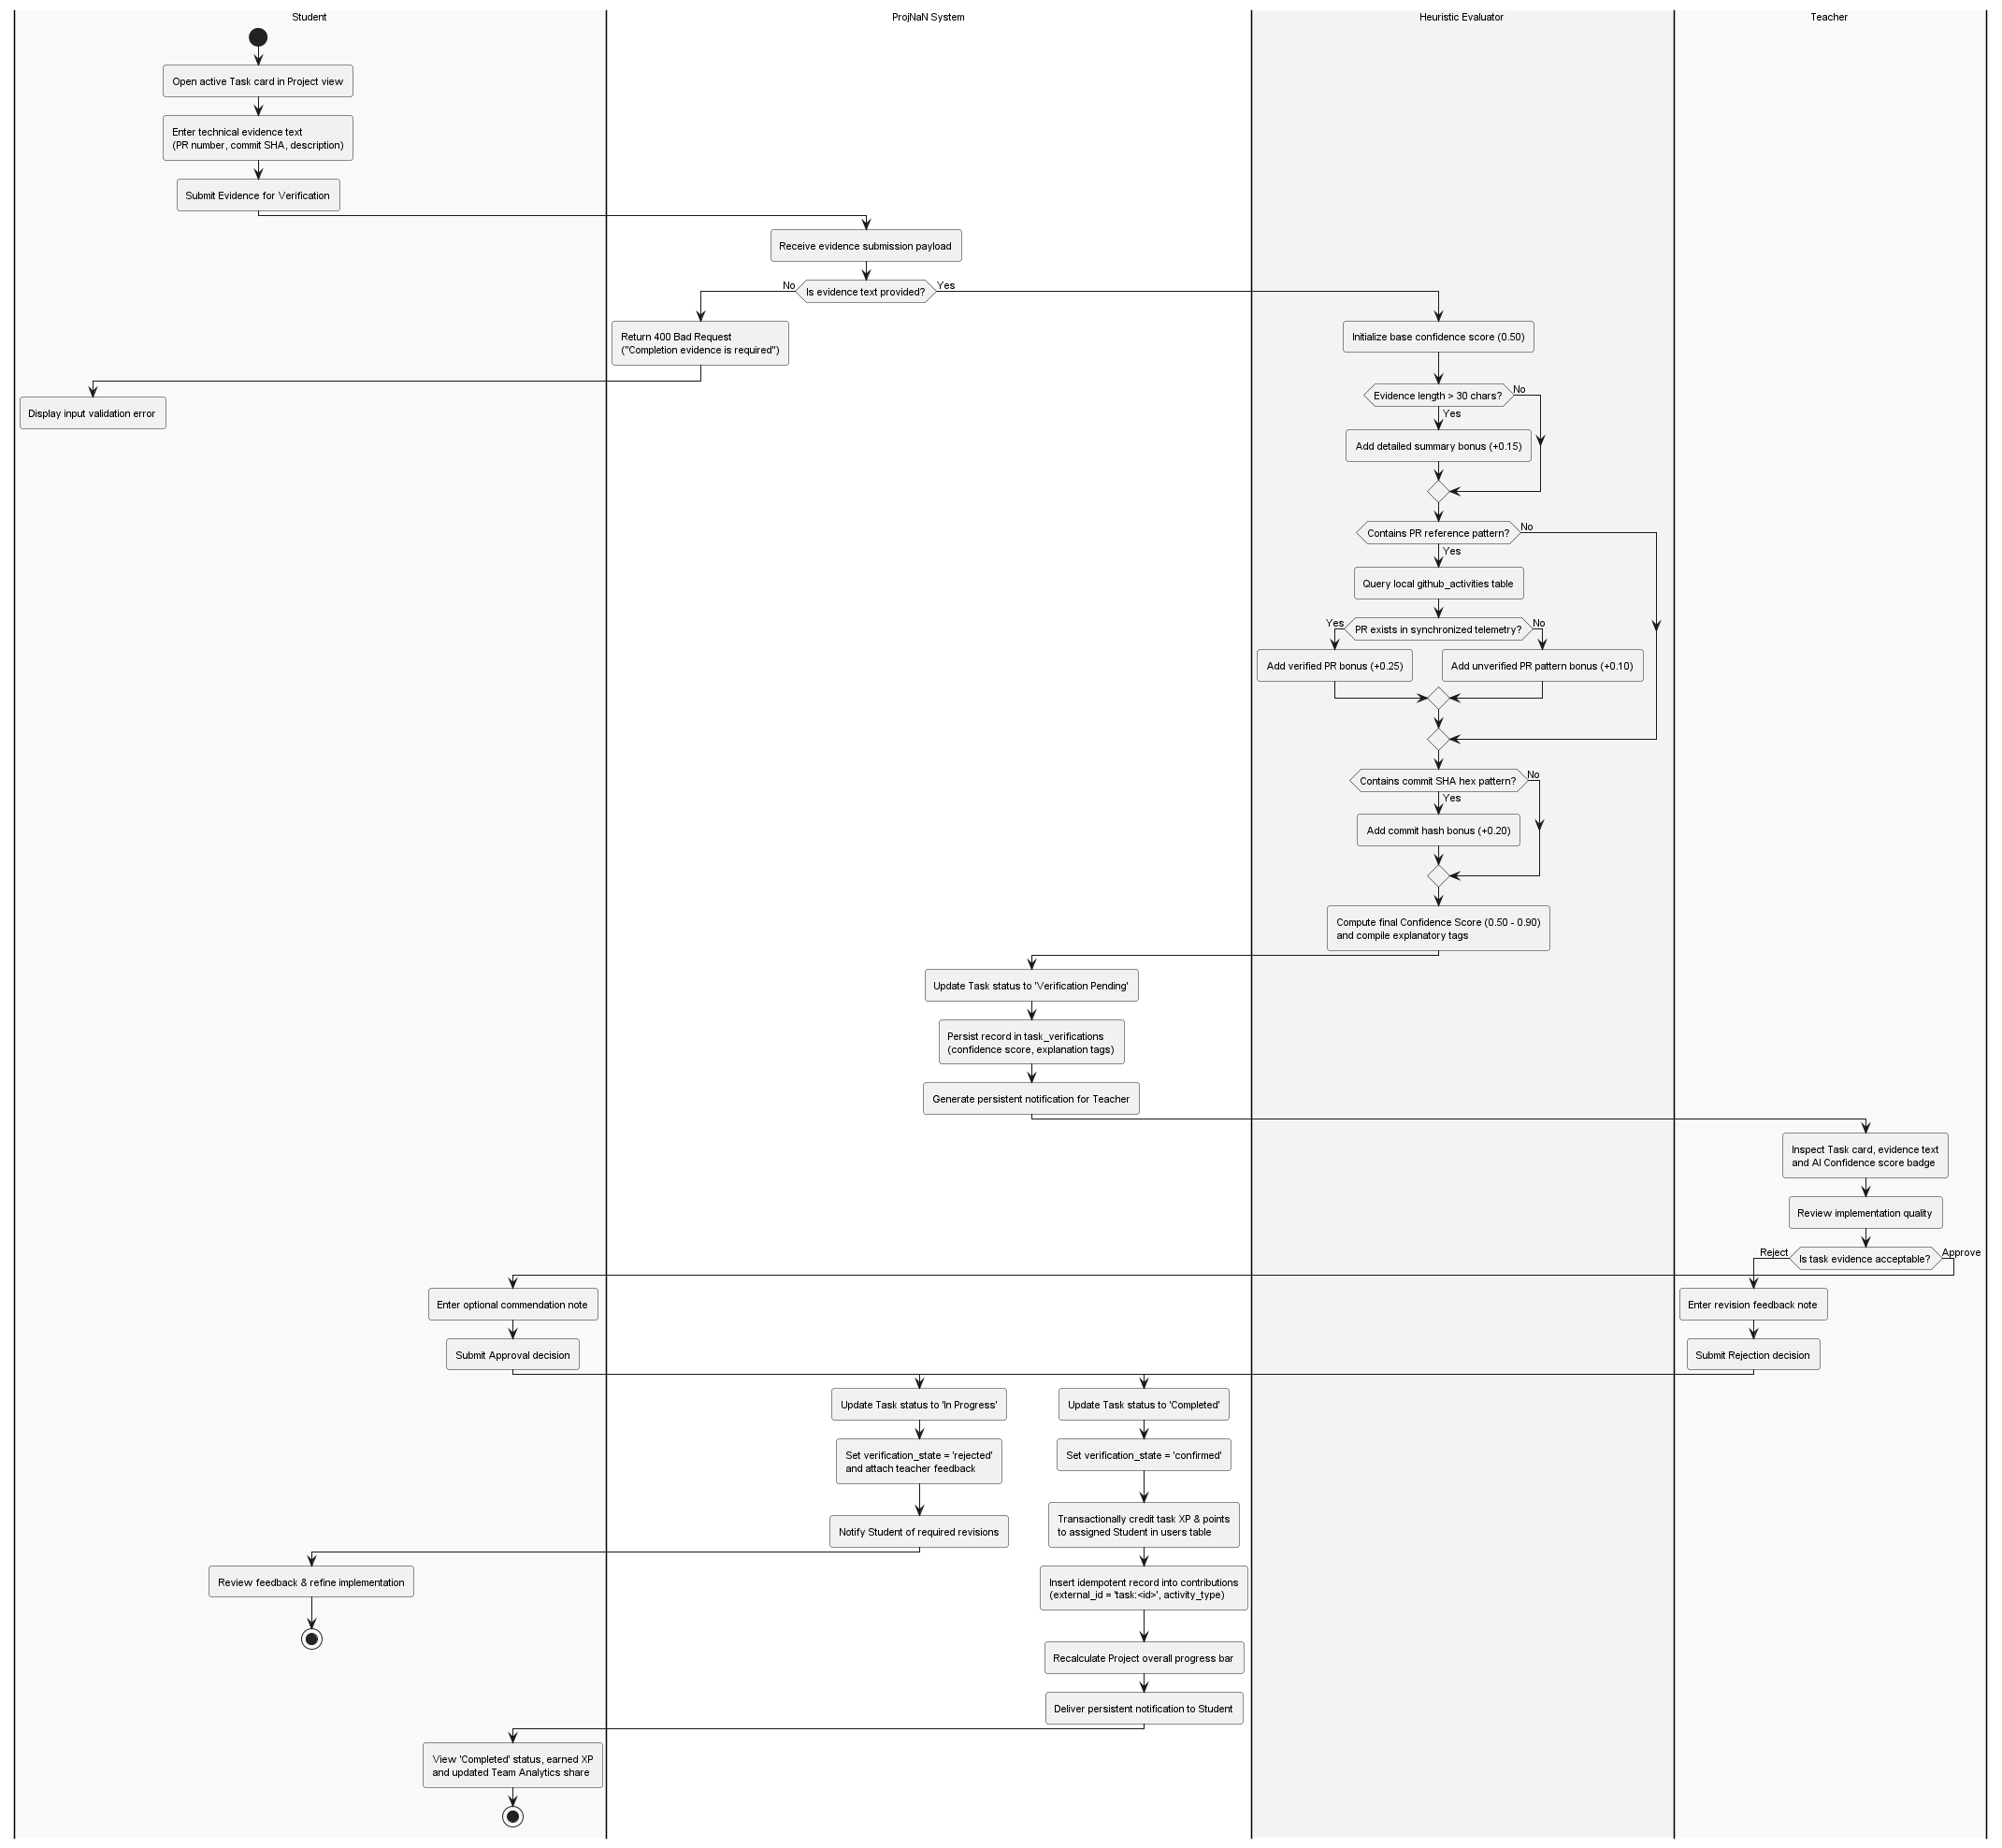
\includegraphics[width=0.88\textwidth]{diagrams/activity.png}
  \caption{Activity Diagram for the Task Evidence Submission and Verification Process}
  \label{fig:activity}
\end{figure}

Figure~\ref{fig:activity} models the process flow across four swimlane partitions (\texttt{Student}, \texttt{ProjNaN System}, \texttt{Heuristic Evaluator}, \texttt{Teacher}). It details input validation, the conditional branching of heuristic score modifiers, the teacher review decision node, and the parallel outcomes: rejection (returning to \texttt{In Progress}) versus approval (awarding XP and logging idempotent contributions).

% ===== CHAPTER 3: RESULTS & EVALUATION =====

\chapter{Results and Evaluation}

\section{Testing Methodology}
The validation strategy combined multi-tiered automated backend test suites, frontend production compilation, and structured security auditing:
\begin{itemize}
  \item \textbf{Unit Testing:} Verification of SQLite schema constraints, cascading deletes, Write-Ahead Logging integrity, and transactional rollbacks.
  \item \textbf{Integration Testing:} End-to-end API testing using Supertest against an Express test instance, validating route status codes, payload handling, and cross-module workflows.
  \item \textbf{Security Auditing:} Dedicated automated tests asserting unauthorized route rejection (e.g., student attempting teacher verification), sliding-window rate limiting, and XSS string stripping.
  \item \textbf{User/Production Build Testing:} Verification via the Vite production build pipeline (\texttt{npm run build}) to confirm zero syntax errors, dead imports, or bundle configuration issues.
\end{itemize}

\section{Performance Metrics}
The system was verified directly against the current repository test and build outputs. All 52 automated backend tests passed with 100\% success across 4 dedicated suites, as summarized in Table~\ref{tab:test_results}.

\begin{table}[H]
\centering
\begin{tabular}{|l|l|r|c|}
  \hline
  \textbf{Test Suite File} & \textbf{Capabilities Verified} & \textbf{Tests} & \textbf{Status} \\
  \hline
  \texttt{auth.test.js} & Registration, login, JWT, email tokens, password reset & 16 & Passed \\
  \texttt{coreWorkflow.test.js} & Classes, teams, tasks, evidence scoring, GitHub sync & 23 & Passed \\
  \texttt{gamification.test.js} & Arena challenges, submissions, leaderboard, badges & 6 & Passed \\
  \texttt{security.test.js} & RBAC teacher guard (403), sanitization, rate limiting & 7 & Passed \\
  \hline
  \textbf{Total Test Suite} & \textbf{Complete System End-to-End Test Suite} & \textbf{52} & \textbf{Passed (52/52)} \\
  \hline
\end{tabular}
\caption{Automated Test Suite Execution Results}
\label{tab:test_results}
\end{table}

System execution measurements verified directly from the production build and test execution environments are presented in Table~\ref{tab:performance}.

\begin{table}[H]
\centering
\begin{tabular}{|l|r|l|}
  \hline
  \textbf{Metric} & \textbf{Verified Measurement} & \textbf{Evaluation Method / Source} \\
  \hline
  Automated Test Pass Rate & $100\%$ (52/52 tests) & \texttt{npm test} across all 4 suites \\
  Test Suite Execution Duration & $\approx 7$ s (observed $6.99$ s) & Node.js native test runner (\texttt{node:test}) \\
  Frontend Production JS Bundle & $390.19$ kB ($106.89$ kB gzip) & Vite production build output (\texttt{dist/}) \\
  Frontend Production CSS Bundle & $29.64$ kB ($6.30$ kB gzip) & Vite production build output (\texttt{dist/}) \\
  Authentication Rate Limiting & Enforced (HTTP 429) & Automated test in \texttt{security.test.js} \\
  Input Sanitization Stripping & Verified ($0$ script injection) & Automated test in \texttt{security.test.js} \\
  Database Response Latency & Not independently benchmarked & Unmeasured under formal load; omitted \\
  \hline
\end{tabular}
\caption{System Performance and Build Verification Results}
\label{tab:performance}
\end{table}

\section{Analysis}
The evaluation confirmed that all primary functional objectives were satisfied:
\begin{itemize}
  \item \textbf{RBAC and Authorization Integrity:} The automated security suite confirmed that student accounts are strictly prohibited from approving task verifications, consistently returning an HTTP 403 Forbidden response.
  \item \textbf{Idempotent Deduplication:} Executing duplicate contribution ingestion with identical external reference keys (\texttt{external\_id}) confirmed that secondary calls are safely ignored without awarding duplicate XP or creating redundant database rows.
  \item \textbf{Fault-Tolerant Telemetry:} Testing GitHub synchronization under simulated network failures verified that the fallback ingestion engine successfully activates, preventing unhandled exceptions or client crashes.
\end{itemize}

% ===== CHAPTER 4: CONCLUSION =====

\chapter{Conclusion}

\section{Summary of Work}
The ProjNaN platform was designed, implemented, and verified as a collaborative project management and contribution verification system for undergraduate software engineering courses. The platform improves visibility and accountability by integrating university course rosters, task lifecycle state machines, automated GitHub synchronization, an internal rule-based heuristic verification engine, and an idempotent contribution ledger with team effort distribution visualizations.

\section{Key Findings}
\begin{itemize}
  \item \textbf{Automated Pre-Checks Assist Faculty Review:} Introducing an internal rule-based heuristic confidence score ($50\% - 90\%$) assists instructors by verifying that PR references and commit hashes exist in repository telemetry prior to manual review.
  \item \textbf{Quantified Effort Distribution Improves Accountability:} Displaying a stacked, multi-colored team effort distribution bar derived from verified contribution records makes individual participation transparent to peers and faculty mentors, discouraging non-participation.
  \item \textbf{Embedded Relational Persistence Simplifies Deployment:} Utilizing SQLite with Write-Ahead Logging delivered reliable ACID transactional safety without requiring separate database server administration.
\end{itemize}

\section{Future Work and Recommendations}
The following architectural extensions are documented as future enhancements:
\begin{enumerate}
  \item \textbf{Large Language Model (LLM) Semantic Diff Analysis:} The current implementation relies on an internal rule-based heuristic evaluator. Integrating external LLM APIs (e.g., Google Gemini 1.5 Pro) would enable automated semantic code reviews of actual Git diffs.
  \item \textbf{Full-Duplex WebSocket Infrastructure:} Upgrading the current REST-based project channel chat to WebSockets (\texttt{socket.io}) to support real-time message streaming.
  \item \textbf{Cross-Project Plagiarism Detection:} Incorporating automated source code similarity algorithms (e.g., MOSS API integration) to cross-check student submissions across academic class cohorts.
\end{enumerate}

\section{Final Remarks}
ProjNaN demonstrates that combining version control telemetry, objective heuristic verification, and gamified contribution tracking improves visibility, accountability, and pedagogical oversight in collaborative software engineering projects.

% ===== BIBLIOGRAPHY =====

% Print bibliography with heading in TOC (Matching TIET template)
\printbibliography[heading=bibintoc]

\end{document}